% Provenance (never printed): the trade strand of ../economics_series.md (grade 9: comparative advantage between
% countries; exports, imports, the trade balance; a tariff as a tax on imports, who gains and who loses; distance and
% transport costs; one paragraph on migration and remittances). Brief: sources/book1/BRIEFS.md, g9-04. Surplus areas
% are grade 10's: the tariff's gains and losses are rectangles of dalens only.
% Chart data: figdata/grade-9/04-international-trade (WDI export mix of South Korea; WDI applied tariffs; WDI
% remittances in facts.csv; invented cloth market; frozen Brenland accounts). Ledger: g9:fht-2020-price-effect,
% g9:fht-2020-dryers.
\chapter{International Trade}\label{ch:g9:international-trade}

\begin{openingchart}{What South Korea sold abroad: each group's share of the value of its exports of goods,
in 1965 and in 2024 (percent).}{World \omterm{def:g8:banks-saving-interest:bank}{Bank}, World Development Indicators}
\begin{tikzpicture}
\begin{axis}[omrecord, xbar, bar width=6pt, width=0.66\linewidth, height=0.42\linewidth, xmin=0, xmax=100,
  ytick=data, yticklabels from table={figdata/grade-9/04-international-trade/out/korea_mix.csv}{group},
  yticklabel style={font=\footnotesize}, enlarge y limits={abs=0.6}, xlabel={Share of exports of goods (percent)},
  nodes near coords, nodes near coords style={font=\scriptsize}, reverse legend,
  legend style={at={(0.97,0.03)}, anchor=south east}, area legend]
\addplot[fill=omDef!40, draw=none] table[x=y1965, y expr=\coordindex]
  {figdata/grade-9/04-international-trade/out/korea_mix.csv};
\addplot[fill=omDef, draw=none] table[x=y2024, y expr=\coordindex]
  {figdata/grade-9/04-international-trade/out/korea_mix.csv};
\legend{1965, 2024}
\end{axis}
\end{tikzpicture}
\end{openingchart}

% figdata: korea_mix (manufactures 59.3 -> 87.3; food 16.7 -> 1.6)
In 1965, food, farm raw materials and ores made up two fifths of what South Korea sold to other countries.
By 2024, manufactured goods were $87.3\,\%$ of its \omterm{def:g6:a-connected-world:export}{exports}, and food was $1.6\,\%$. A country's \omterm{def:g6:a-connected-world:export}{exports} are
not fixed by its soil: they change as its workers, machines and skills change.

\begin{recall}
A country has a \omterm{def:g7:comparative-advantage:comparative-advantage}{comparative advantage} in a good when its \omterm{def:g7:scarcity-and-opportunity-cost:opportunity-cost}{opportunity cost} of that good is lower than the
other country's; both gain when each makes more of the good in which it has its \omterm{def:g7:comparative-advantage:comparative-advantage}{comparative advantage} and
they trade (\cref{ch:g7:comparative-advantage}). \omterm{def:g6:a-connected-world:export}{Exports} are goods and services sold to other countries,
\omterm{def:g6:a-connected-world:import}{imports} those bought from them (\cref{ch:g6:a-connected-world}). With supply and demand lines one finds a
\omterm{def:g7:money:price}{price} and the quantities bought and sold (\cref{ch:g9:demand-and-supply-equations}).
\end{recall}

\section{Comparative advantage between countries}

In \cref{ch:g7:comparative-advantage}, a worker in Brenland needs 4 hours for a roll of cloth and 2 hours
for a sack of grain; in Kestria, 6 hours and 12 hours. Kestria takes longer for both goods, yet it \omterm{def:g7:comparative-advantage:gains-from-trade}{gains from
trade}: a roll of cloth costs it half a sack of grain, against two sacks in Brenland. Kestria has the
\omterm{def:g7:comparative-advantage:comparative-advantage}{comparative advantage} in cloth, Brenland in grain.

\omterm{def:g7:comparative-advantage:comparative-advantage}{Comparative advantage} is not given once and for all. A country whose workers have little schooling and
few machines has its lowest \omterm{def:g7:scarcity-and-opportunity-cost:opportunity-cost}{opportunity costs} in goods made with land and hands; as its workers learn more
and its \omterm{def:g7:firms:firm}{firms} invest, its lowest \omterm{def:g7:scarcity-and-opportunity-cost:opportunity-cost}{opportunity costs} can move to manufactured goods. That is one way to read
the opening chart, but the chart shows the change, not its causes.

\section{Exports, imports and the balance}

\begin{definition}[Trade balance]\label{def:g9:international-trade:trade-balance}
The \emph{trade balance}\index{trade balance} of a country over a year is the value of its \omterm{def:g6:a-connected-world:export}{exports} minus
the value of its \omterm{def:g6:a-connected-world:import}{imports}.
\end{definition}

\begin{definition}[Trade surplus]\label{def:g9:international-trade:trade-surplus}
A country has a \emph{trade surplus}\index{trade surplus} when its \omterm{def:g9:international-trade:trade-balance}{trade balance} is positive: it sells
more to other countries than it buys from them.
\end{definition}

\begin{definition}[Trade deficit]\label{def:g9:international-trade:trade-deficit}
A country has a \emph{trade deficit}\index{trade deficit} when its \omterm{def:g9:international-trade:trade-balance}{trade balance} is negative: it buys more
from other countries than it sells to them.
\end{definition}

A deficit is not a loss, as a \omterm{def:g7:households:household}{household}'s shopping is not a loss: the country gets goods for its \omterm{def:g7:money:money}{money}. A
country with a deficit pays for the difference by borrowing from abroad or by selling assets to foreigners;
a country with a surplus lends or buys assets abroad.

\begin{measure}[The trade balance]
% figdata: brenland (2024 balance -1316, 2025 +1113, with Kestria 2025 +5492)
Customs offices record the goods that cross the border and their value; surveys of \omterm{def:g7:firms:firm}{firms} add services,
such as transport, tourism and banking. In 2024 Brenland exported 125,104 million dalens of goods and
services and imported 126,420 million: a deficit of 1,316 million. In 2025 it had a surplus of 1,113
million. A country can have a surplus with one partner and a deficit with another: the balance that matters
for borrowing is the total.
\end{measure}

\section{What countries sell}

\begin{omfigure}
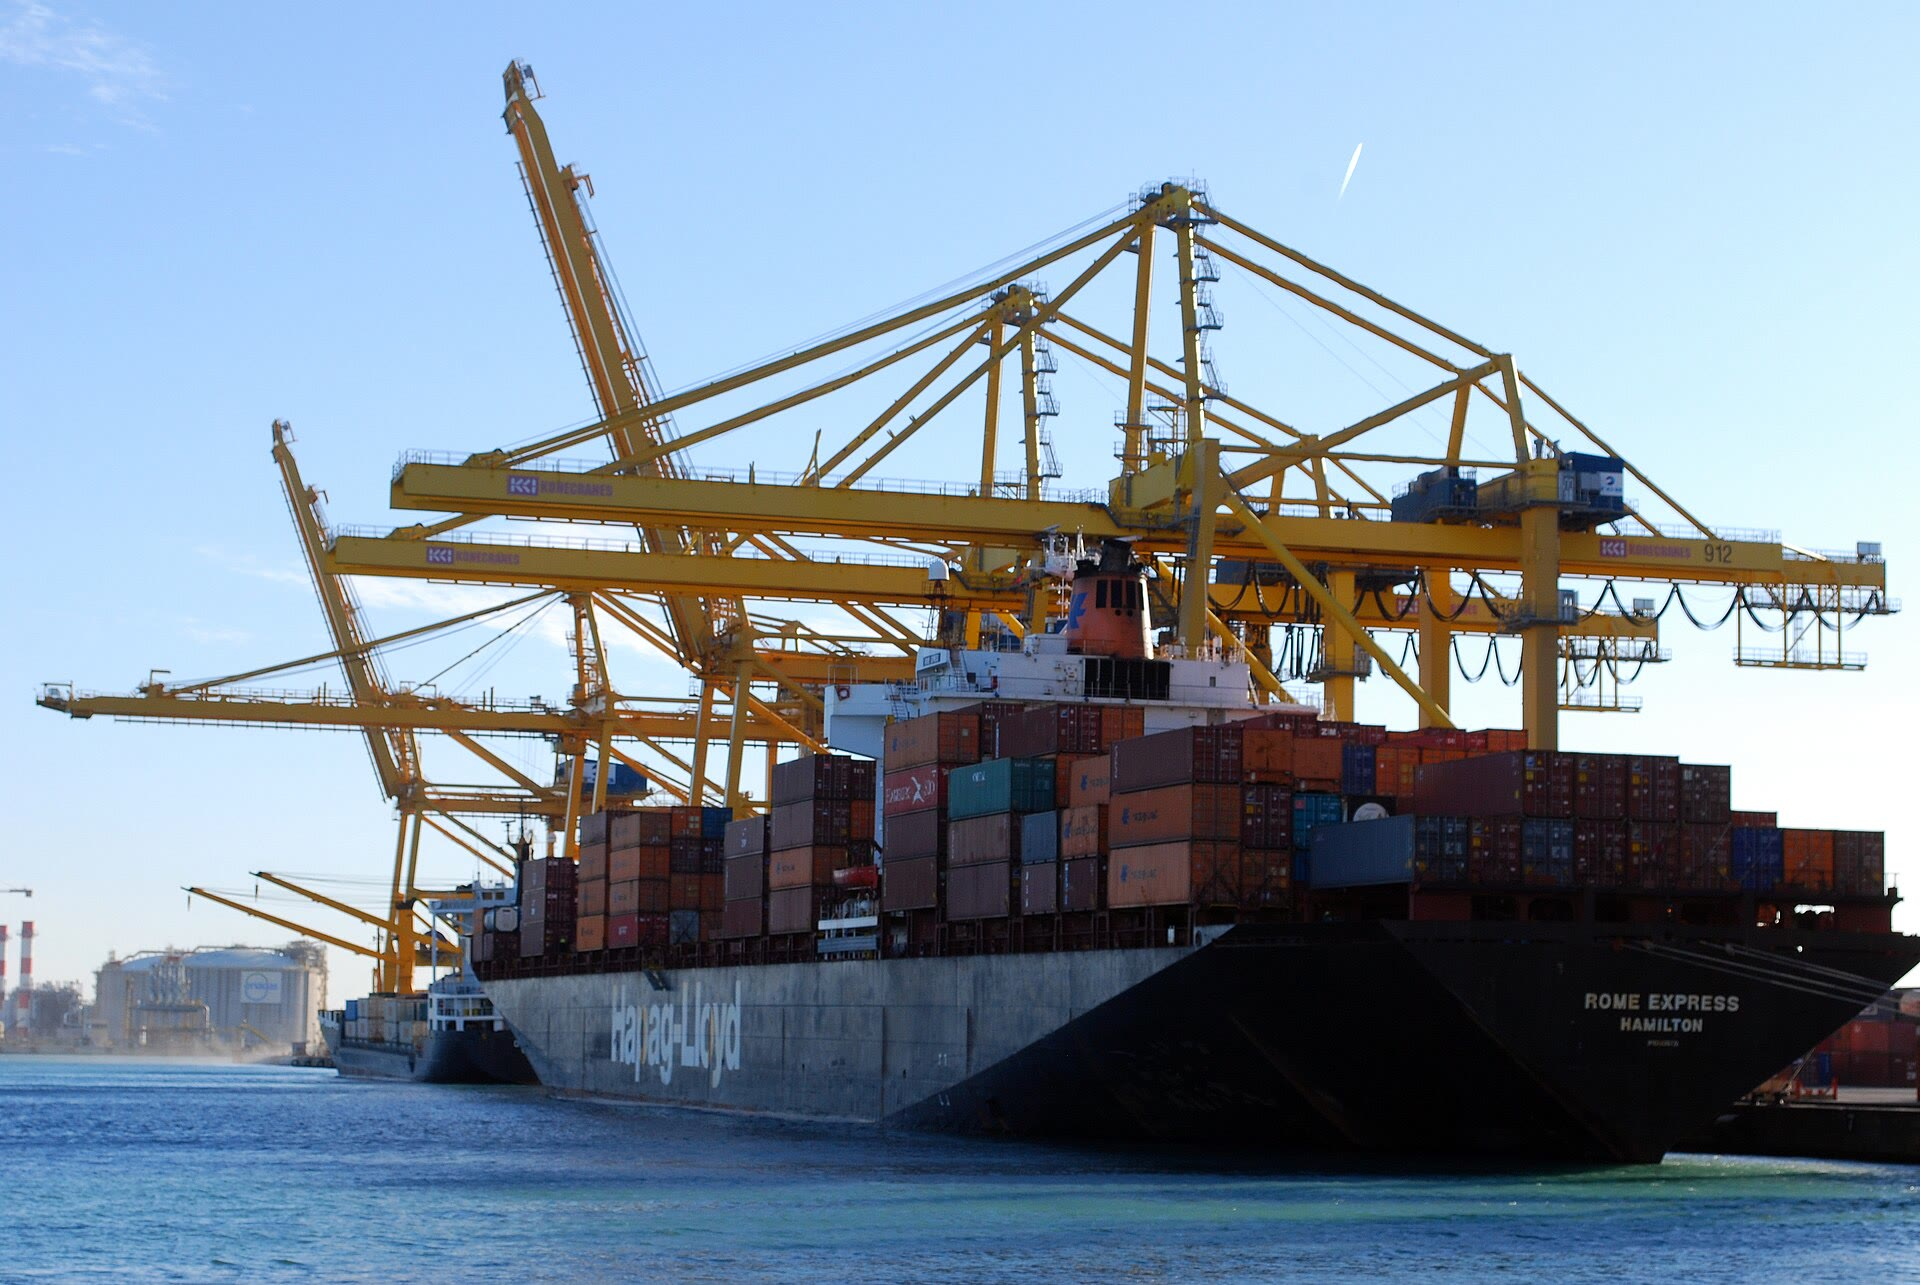
\includegraphics[width=0.62\linewidth]{images/book1/photos/g9-international-trade-container-ship.jpg}

{\small A container ship being loaded in the port of Barcelona, 2010. Photograph: Ivan Mlinaric, CC BY 2.0.}
\end{omfigure}

Countries often sell each other the same kinds of goods: cars go both ways between countries that both
make cars, because each \omterm{def:g7:firms:firm}{firm} makes its own models. Countries also sell each other parts: a good may
cross several borders before it is finished.

% figdata: facts remit_TJK_2024 47.2, remit_PHL_2024 8.7, remit_MEX_2024 3.7, remit_WLD_2024 0.8
People cross borders too. Workers who move abroad often send \omterm{def:g7:money:money}{money} home to their families. In 2024 such
\omterm{def:g7:money:money}{money} was $47.2\,\%$ of the value of all that Tajikistan produced, $8.7\,\%$ in the Philippines and $3.7\,\%$
in Mexico, against $0.8\,\%$ for the world as a whole.

\section{A tariff}

\begin{definition}[Tariff]\label{def:g9:international-trade:tariff}
A \emph{tariff}\index{tariff} is a \omterm{def:g8:taxes-and-public-spending:tax}{tax} on imported goods.
\end{definition}

\begin{definition}[Import quota]\label{def:g9:international-trade:import-quota}
An \emph{import quota}\index{import quota} is a legal limit on the quantity of a good that may be
imported.
\end{definition}

% figdata: tariffs (first and 2022 values in facts.csv)
\begin{omchart}{Average tariff on imports, weighted by what each economy imports: five economies (percent).
Years with no value are left blank.}{World \omterm{def:g8:banks-saving-interest:bank}{Bank}, World Development Indicators; the United States
value for 2019 (13.8) is left out as a break in the series}
\begin{tikzpicture}
\begin{axis}[omrecord, width=0.9\linewidth, height=0.45\linewidth, xmin=1988, xmax=2022, ymin=0, ymax=60,
  xlabel={Year}, ylabel={Tariff (percent)}, unbounded coords=jump, legend columns=5,
  xtick={1990,1995,...,2020}, xticklabel style={/pgf/number format/1000 sep={}},
  legend style={at={(0.5,1.03)}, anchor=south, font=\footnotesize}, mark size=1pt]
\addplot[omDef, thick, mark=*] table[x=year, y=IND] {figdata/grade-9/04-international-trade/out/tariffs.csv};
\addplot[omThm, thick, mark=*] table[x=year, y=CHN] {figdata/grade-9/04-international-trade/out/tariffs.csv};
\addplot[black!70, thick, mark=*] table[x=year, y=BRA] {figdata/grade-9/04-international-trade/out/tariffs.csv};
\addplot[omDef!50, thick, dashed, mark=*] table[x=year, y=USA] {figdata/grade-9/04-international-trade/out/tariffs.csv};
\addplot[omThm!50, thick, dashed, mark=*] table[x=year, y=EUU] {figdata/grade-9/04-international-trade/out/tariffs.csv};
\legend{India, China, Brazil, United States, European Union}
\end{axis}
\end{tikzpicture}
\end{omchart}

India's average \omterm{def:g9:international-trade:tariff}{tariff} was $56\,\%$ in 1990 and $4.6\,\%$ in 2022; China's $32\,\%$ in 1992 and $2.2\,\%$ in
2022. In the United States and the European Union, \omterm{def:g9:international-trade:tariff}{tariffs} were already low in 1990.

Take Brenland's \omterm{def:g7:markets-and-prices:market}{market} for cloth, a small part of the world \omterm{def:g7:markets-and-prices:market}{market}: whatever Brenland buys, the world \omterm{def:g7:money:price}{price}
stays at 6 dalens a metre. Brenland's buyers want $Q^d = 100 - 5p$ thousand metres a year and its weavers
offer $Q^s = 5p - 10$. Without trade the \omterm{def:g7:money:price}{price} would be 11 dalens, where $100 - 55 = 55 - 10 = 45$. With trade,
the \omterm{def:g7:money:price}{price} at home is the world \omterm{def:g7:money:price}{price}: buyers want 70, weavers make 20, and 50 are imported.

With a \omterm{def:g9:international-trade:tariff}{tariff} of 2 dalens a metre, an imported metre costs $6 + 2 = 8$ dalens at home, and Brenland's weavers
can sell at 8 too. Buyers want $100 - 40 = 60$, weavers make $40 - 10 = 30$, and \omterm{def:g6:a-connected-world:import}{imports} fall to 30. The state
collects $2 \times 30 = 60$ thousand dalens.

\begin{omchart}{Brenland's cloth market, a small country, with a world price of 6 dalens a metre and a
tariff of 2 dalens (invented). Imports are the gap between the two lines at the price paid at home: 50
without the tariff, 30 with it.}{Invented}
\begin{tikzpicture}
\begin{axis}[omrecord, xmin=0, xmax=100, ymin=0, ymax=20, height=0.5\linewidth, width=0.8\linewidth,
  xlabel={Thousand metres a year}, ylabel={Price (dalens a metre)}, xtick={0,20,30,45,60,70,100},
  ytick={0,6,8,11,20}]
\addplot[demand] table[x=qd, y=price] {figdata/grade-9/04-international-trade/out/cloth.csv};
\addplot[supply] table[x=qs, y=price] {figdata/grade-9/04-international-trade/out/cloth.csv};
\draw[thick, black] (axis cs:0,6) -- (axis cs:100,6) node[pos=0.88, below, font=\scriptsize] {world price};
\draw[thick, black, dashed] (axis cs:0,8) -- (axis cs:100,8) node[pos=0.88, above, font=\scriptsize] {with the tariff};
\draw[<->, thick, omThm] (axis cs:20,4.5) -- (axis cs:70,4.5) node[midway, below, font=\scriptsize] {imports 50};
\draw[<->, thick, omThm] (axis cs:30,8.7) -- (axis cs:60,8.7) node[right, font=\scriptsize] {imports 30};
\draw[guide] (axis cs:20,6) -- (axis cs:20,0);
\draw[guide] (axis cs:70,6) -- (axis cs:70,0);
\draw[guide] (axis cs:30,8) -- (axis cs:30,0);
\draw[guide] (axis cs:60,8) -- (axis cs:60,0);
\draw[guide] (axis cs:0,11) -- (axis cs:45,11) -- (axis cs:45,0);
\node[anchor=west, font=\footnotesize, text=omDef] at (axis cs:12,19) {demand};
\node[anchor=west, font=\footnotesize, text=omThm] at (axis cs:80,19) {supply};
\end{axis}
\end{tikzpicture}
\end{omchart}

Who gains and who loses? Buyers pay 2 dalens more on each of the 60 thousand metres they still buy: 120
thousand dalens a year. Of that, 60 go to the state and $2 \times 30 = 60$ to Brenland's weavers. Every
dalen that buyers pay extra on those metres goes to someone at home. But the \omterm{def:g9:international-trade:tariff}{tariff} also costs something
that nobody receives: buyers give up 10 thousand metres they would have bought at 6 dalens, and weavers make
10 thousand more metres at a cost above 6 dalens, when the same cloth could be bought abroad for 6.

\begin{model}{A tariff in a small country}
\assumes The country's buyers are too few to move the world \omterm{def:g7:money:price}{price}; many sellers at home and abroad.
\predicts The home \omterm{def:g7:money:price}{price} rises by the \omterm{def:g9:international-trade:tariff}{tariff}; \omterm{def:g6:a-connected-world:import}{imports} fall; home producers sell more and at a higher
\omterm{def:g7:money:price}{price}; the state collects \omterm{def:g7:firms:revenue}{revenue}; home buyers lose more than producers and the state gain.
\tested Consistent with it: after the 2018 United States \omterm{def:g9:international-trade:tariff}{tariffs} on imported washing machines, the home
\omterm{def:g7:money:price}{price} of washers rose by nearly $12\,\%$ (Flaaen, Hortaçsu and Tintelnot, 2020). It is not a test of the
small-country model: the United States is a large buyer, the case the next field sets aside. A test
would need a small country's \omterm{def:g9:international-trade:tariff}{tariff}, with its rate set beside the rise in the home \omterm{def:g7:money:price}{price}.
\breaks A large country's buyers can push down the world \omterm{def:g7:money:price}{price}, so part of the \omterm{def:g9:international-trade:tariff}{tariff} falls on foreign
sellers; other countries may answer with \omterm{def:g9:international-trade:tariff}{tariffs} of their own; sellers of related goods may raise their
\omterm{def:g7:money:price}{prices} too.
\end{model}
% ledger: g9:fht-2020-price-effect

\begin{record}[Washing machines, 2018]
% ledger: g9:fht-2020-price-effect, g9:fht-2020-dryers
In 2018 the United States put \omterm{def:g9:international-trade:tariff}{tariffs} on imported washing machines. A study found that the \omterm{def:g7:money:price}{price} of
washers rose by nearly $12\,\%$, and that the \omterm{def:g7:money:price}{price} of dryers, which were not taxed and are often bought
together with a washer, rose by about as much (Flaaen, Hortaçsu and Tintelnot, 2020). The
buyers of dryers paid more too, although the \omterm{def:g9:international-trade:tariff}{tariff} did not name dryers.
\end{record}

\section{Distance}

Moving goods costs \omterm{def:g7:money:money}{money}. A transport cost works like a \omterm{def:g9:international-trade:tariff}{tariff}: it raises the home \omterm{def:g7:money:price}{price} of an imported
good above its \omterm{def:g7:money:price}{price} where it is made. Unlike a \omterm{def:g9:international-trade:tariff}{tariff}, it brings no \omterm{def:g7:firms:revenue}{revenue} to the state: the \omterm{def:g7:money:money}{money} pays
for ships, fuel and work. When transport costs fall, imported goods become cheaper at home, and exporters
can sell more abroad. Containers, which go from ship to train to lorry without being opened, cut the cost
of loading and unloading.

For the same reason, countries tend to trade more with near countries than with far ones. In Brenland's
accounts, about three tenths of its \omterm{def:g6:a-connected-world:export}{exports} go to Kestria, its neighbour.

\section{Exercises}

\begin{exercise}[$\star$]\label{exo:g9:international-trade:1}
Use the opening chart. What share of South Korea's \omterm{def:g6:a-connected-world:export}{exports} of goods were manufactures in 1965 and in
2024?
\end{exercise}

\begin{exercise}[$\star$]\label{exo:g9:international-trade:2}
A country \omterm{def:g6:a-connected-world:export}{exports} 450 million dalens of goods and services in a year and \omterm{def:g6:a-connected-world:import}{imports} 520 million. Compute its
\omterm{def:g9:international-trade:trade-balance}{trade balance}. Is it a surplus or a deficit?
\end{exercise}

\begin{exercise}[$\star$]\label{exo:g9:international-trade:3}
Use the \omterm{def:g9:international-trade:tariff}{tariff} chart. Read India's average \omterm{def:g9:international-trade:tariff}{tariff} in 1990 and in 2022.
\end{exercise}

\begin{exercise}[$\star$]\label{exo:g9:international-trade:4}
The world \omterm{def:g7:money:price}{price} of a bicycle is 150 dalens. Brenland, a small country, puts a \omterm{def:g9:international-trade:tariff}{tariff} of 30 dalens on each
imported bicycle. What is the \omterm{def:g7:money:price}{price} of a bicycle in Brenland?
\end{exercise}

\begin{exercise}[$\star\star$]\label{exo:g9:international-trade:5}
In Brenland's cloth \omterm{def:g7:markets-and-prices:market}{market} ($Q^d = 100 - 5p$, $Q^s = 5p - 10$, world \omterm{def:g7:money:price}{price} 6), compute \omterm{def:g6:a-connected-world:import}{imports} without a
\omterm{def:g9:international-trade:tariff}{tariff} and with a \omterm{def:g9:international-trade:tariff}{tariff} of 3 dalens a metre.
\end{exercise}

\begin{exercise}[$\star\star$]\label{exo:g9:international-trade:6}
Compute the state's \omterm{def:g7:firms:revenue}{revenue} from the \omterm{def:g9:international-trade:tariff}{tariff} of 3 dalens in exercise 5.
\end{exercise}

\begin{exercise}[$\star\star$]\label{exo:g9:international-trade:7}
In Brenland's cloth \omterm{def:g7:markets-and-prices:market}{market}, the \omterm{def:g9:international-trade:tariff}{tariff} doubles from 2 to 4 dalens a metre. What happens to the home \omterm{def:g7:money:price}{price}
and to \omterm{def:g6:a-connected-world:import}{imports}? Do \omterm{def:g6:a-connected-world:import}{imports} halve?
\end{exercise}

\begin{exercise}[$\star\star$]\label{exo:g9:international-trade:8}
In 2025 Brenland sold 40,231 million dalens of goods and services to Kestria and bought 34,739 million from
it. Its total \omterm{def:g6:a-connected-world:export}{exports} were 129,777 million and its total \omterm{def:g6:a-connected-world:import}{imports} 128,664 million. Compute its balance with
Kestria and its total balance.
\end{exercise}

\begin{exercise}[$\star\star$]\label{exo:g9:international-trade:9}
A country puts a \omterm{def:g9:international-trade:tariff}{tariff} on a good, and the world \omterm{def:g7:money:price}{price} of the good falls by half the \omterm{def:g9:international-trade:tariff}{tariff}. Which
assumption of the \omterm{def:g9:international-trade:tariff}{tariff} model does this observation contradict? What kind of country is it likely to
be?
\end{exercise}

\begin{exercise}[$\star\star\star$]\label{exo:g9:international-trade:10}
In Brenland's cloth \omterm{def:g7:markets-and-prices:market}{market} with a \omterm{def:g9:international-trade:tariff}{tariff} of 3 dalens a metre (exercise 5), compute how much more buyers pay
on the metres they still buy, how much more weavers receive on the metres they sell, and the state's
\omterm{def:g7:firms:revenue}{revenue}. Check that the first is the sum of the other two.
\end{exercise}

\begin{exercise}[$\star\star\star$]\label{exo:g9:international-trade:11}
The cost of shipping goods between two countries halves. What happens to the \omterm{def:g7:money:price}{prices} of imported goods in
each country, to the quantity traded, and to the producers of the imported goods in each country?
\end{exercise}

\begin{exercise}[$\star\star\star$]\label{exo:g9:international-trade:12}
What can the opening chart not tell you about why South Korea's \omterm{def:g6:a-connected-world:export}{exports} changed? Name two possible causes
that the chart cannot tell apart.
\end{exercise}

\section{Problem: A Tariff on Kestrian Cloth}

\begin{problem}[{Weekend problem --- Brenland's cloth market and the world price, a tariff on imported
cloth, and who gains and who loses}]
\label{pb:g9:international-trade:1}
Everything in this problem is invented. In a fine-cloth \omterm{def:g7:markets-and-prices:market}{market}, Brenland's buyers want $Q^d = 900 - 30p$
thousand metres a year at a \omterm{def:g7:money:price}{price} of $p$ dalens a metre, and its weavers offer $Q^s = 20p - 100$. Kestria
and other countries sell any quantity to Brenland at the world \omterm{def:g7:money:price}{price} of 10 dalens a metre.

\medskip
\noindent\textbf{Part I --- Without a tariff.}
\begin{enumerate}
  \item Compute the quantities demanded and supplied at 10 and at 20 dalens.
  \item Without any trade, what would the \omterm{def:g7:money:price}{price} and the quantity be?
  \item With trade at the world \omterm{def:g7:money:price}{price}, how much does Brenland \omterm{def:g6:a-connected-world:import}{import}?
  \item What is the weavers' \omterm{def:g7:firms:revenue}{revenue} at the world \omterm{def:g7:money:price}{price}?
\end{enumerate}

\medskip
\noindent\textbf{Part II --- A tariff of 4 dalens a metre.}
\begin{enumerate}[resume]
  \item What is the \omterm{def:g7:money:price}{price} of cloth in Brenland?
  \item Compute the quantities demanded and supplied at that \omterm{def:g7:money:price}{price}.
  \item Compute the \omterm{def:g6:a-connected-world:import}{imports}.
  \item Compute the state's \omterm{def:g7:firms:revenue}{revenue} from the \omterm{def:g9:international-trade:tariff}{tariff}.
\end{enumerate}

\medskip
\noindent\textbf{Part III --- Who gains and who loses.}
\begin{enumerate}[resume]
  \item How much more do buyers pay on the metres they still buy?
  \item How much more do weavers receive on the metres they sell, compared with selling the same metres
        at 10 dalens?
  \item Compare the answer to question 9 with the sum of the answers to questions 8 and 10.
  \item How many metres do buyers no longer buy? How many more metres do Brenland's weavers make?
  \item Explain why buyers lose more than the weavers and the state gain.
\end{enumerate}
\end{problem}
